%-----------------------------------------------------------------------------%
%                            Set Page STYLE                                   %
%-----------------------------------------------------------------------------%

% THIS IS THE DEFAULT PAGE STYLE
\pagestyle{fancy}
\fancyhf{}
\renewcommand{\footrulewidth}{0pt}
\fancyfoot[R]{\textbf{\thepage}}
\fancyfoot[L]{$subtitle$}
\renewcommand{\footrulewidth}{1pt}

% THE TABLE OF CONTENTS PAGE USES THIS STYLE
\fancypagestyle{plain}{%
  \renewcommand{\headrulewidth}{0pt}%
  \fancyhf{}%
  \renewcommand{\footrulewidth}{1pt}
  \fancyfoot[R]{\textbf{\thepage}}%
  % THE TITLE IS NOT ACTUALLY GOING HERE WHY??
  \fancyfoot[L]{$subtitle$} % HERE GOES THE TITLE
}

% IT IS ALSO POSSIBLE TO USE STYLE empty AS IN THE TITLE PAGE AND FINAL PAGE

%-----------------------------------------------------------------------------%
% START OF TITLE PAGE
%-----------------------------------------------------------------------------%
\thispagestyle{empty}

% Define a dimension for the height of the banner for the title page
\newdimen\bannerheight

% Set \bannerheight to the height of the banner
\settoheight{\bannerheight}{%
  
\includegraphics[width=\paperwidth]{images/title-banner.png}%
}

% Title banner top
\AddToShipoutPictureBG*{%
 \AtPageUpperLeft{\raisebox{-\height}{
\includegraphics[width=\paperwidth]{images/title-banner.png}}}
 }

% Cover picture
\AddToShipoutPictureBG*{%
 %\AtPageLowerLeft{\raisebox{0.5\height}{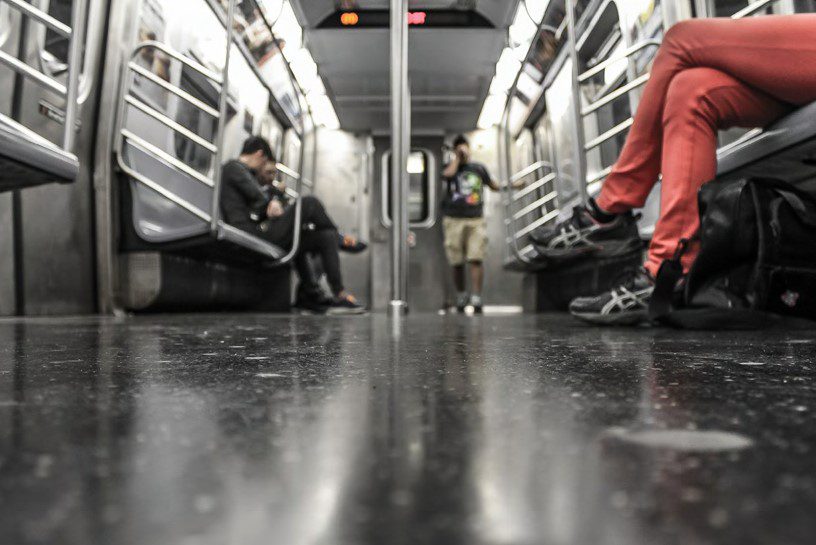
\includegraphics[width=\paperwidth]{images/cover-picture.png}}}
 \AtPageUpperLeft{\raisebox{-\bannerheight-\height}{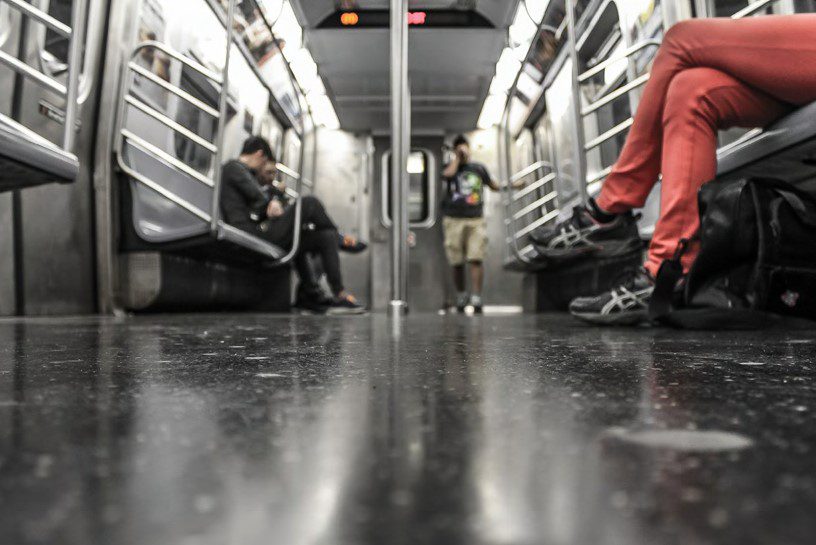
\includegraphics[width=\paperwidth]{images/cover-picture.png}}}
 }

% HERE GOES THE TITLE OF THE DOCUMENT
$if(title)$
  \vspace{-5cm}{\relscale{1.75}{\textcolor{white}{$title$}}}\par%
$endif$
% HERE GOES THE DOCUMENT TYPE; CURRENTLY HARDCODED BUT COULD BE AN INPUT IN template.qmd
{\relscale{1.25}{\textcolor{Yellow}{Report}}}\hfill
% HERE GOES THE DATE OF PUBLICATION
{\relscale{1.0}{\textcolor{LightGray}{$date$}}}
        
% Report information: Needs information that is in file template.qmd
\begin{flushleft}
  \vspace{0.5cm} 
  % HERE GO THE AUTHORS AFFILIATIONS (ONLY NAME OF ORGANIZATION)
  % Needs to iterate by authors
  $for(by-author)$
    {\relscale{1.25}{\textcolor{Yellow}{$by-author.name.literal$}}} 
    % Needs to iterate by affilitations
    $for(by-author.affiliations)$
      \hskip 10pt{\relscale{0.75}{\textcolor{LigghtGray}{$by-author.affiliations.name$}}} \par%
    $endfor$ 
  $endfor$
\end{flushleft}

% Mobilizing Justice Logo
\AddToShipoutPictureBG*{\put(50,30)%
{
\includegraphics[width=0.5\textwidth]{images/mj-logo.png}%
}}

%-----------------------------------------------------------------------------%
% END OF TITLE PAGE
%-----------------------------------------------------------------------------%
\newpage

%-----------------------------------------------------------------------------%
% START OF ABOUT PAGE
%-----------------------------------------------------------------------------%

\section*{About Mobilizing Justice}

The Mobilizing Justice Partnership is funded by the Social Sciences and Humanities Research Council (SSHRC). Based at the University of Toronto Scarborough, the national intersectoral research partnership aims to understand and address transportation poverty in Canada and to improve the well-being of Canadians at risk of transport poverty. Learn more at \url{www.mobilizingjustice.ca}.

% TABLE OF PARTNERS

\section*{Our Partners}
\begin{center}
\ctable[
%label = width,
width = \textwidth,
pos = ht,
left,
doinside = \relscale{0.87}{}
]{| >{\setlength{\baselineskip}{0.1\baselineskip}}>{\raggedright}X | >{\setlength{\baselineskip}{0.1\baselineskip}}>{\raggedright}X | >{\setlength{\baselineskip}{0.1\baselineskip}}>{\raggedright}X |}{}
{ \FL
Amalgamated Transit Union Canada                                                & Infrastructure Canada              & Transit App                                \LL
Autorité régionale de transport métropolitain (ARTM)                            & McGill University                  & TransLink                      \LL
Canadian Institute of Planners                                                  & McMaster University                & United   Way Greater Toronto   \LL
Canada Mortgage and Housing Corporation (CMHC)                                  & Memorial University                & University of British Columbia \LL
Canadian Urban Institute                                                        & Metrolinx                          & University of Manitoba         \LL
Canadian Urban Transit Association                                              & Ontario Ministry of Transportation & University of Oregon           \LL
The Centre for Active Transportation (TCAT), a project of Clean Air Partnership & Pantonium                          & University of Texas Austin     \LL
CIRODD (École de technologie supérieure)                                        & Pembina Institute                  & University of Toronto          \LL
CIRRELT (Université de Montréal)                                                & Region of Waterloo                 & University of Waterloo         \LL
City of Calgary                                                                 & RideShark                          & Urban Strategies               \LL
City of Edmonton                                                                & Simon Fraser University            & Via Transportation Inc.        \LL
City of Toronto                                                                 & Spare Labs                         & Ville de Montréal              \LL
City of Vancouver                                                               & SPIN                               & York Region                    \LL
Esri Canada                                                                     & Statistics Canada                  &    \LL
Federation of Canadian Municipalities	& Toronto Transit Commission (TTC)	& \LL
}
\end{center}

%-----------------------------------------------------------------------------%
% END OF ABOUT PAGE
%-----------------------------------------------------------------------------%
\newpage

%-----------------------------------------------------------------------------%
% START OF AUTHORS PAGE
%-----------------------------------------------------------------------------%

\section*{About the Author(s)}

$for(by-author)$
  {\relscale{1.25}{\textcolor{Maroon}{$by-author.name.literal$}}}%
  % Needs to iterate by affilitations department
  $for(by-author.affiliations)$
    \vskip 1pt{\relscale{0.75}{\textcolor{black}{$by-author.affiliations.department$}}}%
  $endfor$ 
  % Needs to iterate by affilitations name
  $for(by-author.affiliations)$
    \vskip -8pt{\relscale{0.75}{\textcolor{black}{$by-author.affiliations.name$}}}%
  $endfor$ 
  % Needs to iterate by email
  $for(by-author.email)$
    \vskip -8pt{\relscale{0.75}{\textcolor{black}{email: \url{$by-author.email$}}}}%
  $endfor$ 
  \vskip 15pt
$endfor$

%-----------------------------------------------------------------------------%
% END OF AUTHORS PAGE
%-----------------------------------------------------------------------------%
\newpage

%-----------------------------------------------------------------------------%
% START OF ACKNOWLEDGMENTS PAGE
%-----------------------------------------------------------------------------%

\section*{Acknowledgements}

$if(acknowledgements)$
  $acknowledgements$
$endif$

%-----------------------------------------------------------------------------%
% END OF ACKNOWLEDGMENTS PAGE
%-----------------------------------------------------------------------------%
\newpage

%-----------------------------------------------------------------------------%
% START OF TABLE OF CONTENTS PAGE
%-----------------------------------------------------------------------------%

% Table of contents picture top
\AddToShipoutPictureBG*{%
 \AtPageUpperLeft{\raisebox{-\height}{\includegraphics[width=\paperwidth]{images/table-of-contents-picture.png}}}}

% Change the geometry of this one page so that the table of contents begins below the banner image instead of on top of it
\newgeometry{top=10cm}

% Title for the table of contents
%\renewcommand\contentsname{\color{DarkBlue}\normalfont\bfseries\fontsize{24}{28.8}\selectfont Table of Contents}
%\restoregeometry
%\newgeometry{left=5cm}
\setcounter{tocdepth}{1}
\tableofcontents
\restoregeometry

%-----------------------------------------------------------------------------%
% END OF TABLE OF CONTENTS
%-----------------------------------------------------------------------------%
\newpage